\documentclass{article}
\usepackage[utf8]{inputenc}
\title{Video 2: the central limit theorem}
\author{wbg231 }
\date{December 2022}
\newcommand{\R}{$\mathbb{R}$}
\newcommand{\B}{$\beta$}
\newcommand{\A}{$\alpha$}
\newcommand{\D}{\Delta}

\newcommand{\avector}[2]{(#1_2,\ldots,#1_{#2})}
\newcommand{\makedef}[2]{$\textbf{#1}$:#2 }
\usepackage{tikz,graphicx,hyperref,amsmath,amsfonts,amscd,amssymb,bm,cite,epsfig,epsf,url}

\begin{document}

\maketitle

\section{introduction}
\begin{itemize}
\item \href{https://www.youtube.com/watch?v=0z4rGGcvN2Y&list=PLBEf5mJtE6KuZ5NBQMuWIMsiOOrV9ibzm&index=71}{video link}
\item today we are talking about the central limit theorem 
\section{law of large numbers review}
\item if $\Tilde{x}_1...$ are independent  random warbles with mean $\mu$ and variance $\sigma^2$
\item the sample mean $\Tilde{m}_{n}=\frac{1}{n}\Sigma_{i=1}^{n}\Tilde{x}_i$
\item $E[\Tilde{m}_{n}]=\mu$ by linearity of expectations 
\item and $var(\Tilde{m}_n)=\frac{\sigma^2}{m}$ by Independence and linearity of expectations
\item further $P(|\Tilde{m}_{n} -\mu\|> \epsilon)\leq \frac{\sigma^2}{n\epsilon^2}$ meaning the sample mean is consistent, and as our sample size approaches infinity, the chance that it deviates from the population mean approach 0
\item so as we average over more and more samples we can see that the sample means as n grows are confined to be $\epsilon$ close to the population mean 
\item but this does not tell us what the behavior of this sample mean is for a fixed n and this is what we do with the central limit theorem 
\section{central limit theorem}
\subsection{Gorbachev's bound}
\item chebychevs bound gives us $P(|\Tilde{m}_{n}-\mu_{pop}|>\epsilon)\leq \frac{\sigma^2_{pop}}{n\epsilon^2}$ 
\item we can compare this to the empirical probability we get from monte carlo methods, and see how good the law of large numbers is at approximating the distance of the sample mean and population mean 
\item it is a pretty louse bound and a bad approximation 
\item 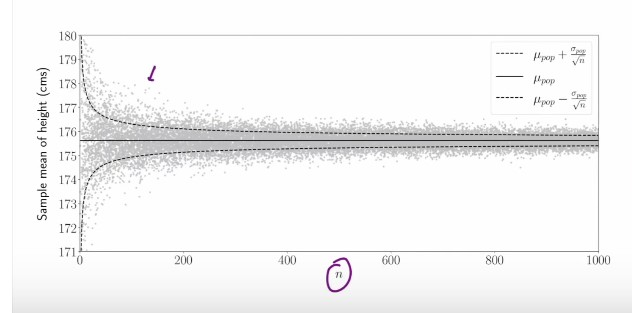
\includegraphics[width=10cm]{notes/week_3/Video 2: the standard error/immages/v_2_1.jpg}
\item so the law of large numbers does not provide a good estimate of the behavior of the sample mean for a fixed value of n 
\subsection{goal}
\item our goal is to approximate the distribution of the sample mean for a fixed n $\Tilde{m}_{n}=\frac{1}{n}\Sigma_{i=1}^{n}\Tilde{x}_i$
\subsection{the sum of discrete rv}
\item let $\Tilde{s}=\Tilde{a}+\Tilde{b}$
\item $P_{\Tilde{s}}(s)=\Sigma_{i=-\infty}^{\infty}P_{\Tilde{a}}(a)p_{\Tilde{b}}(s-a)=p_{\Tilde{a}}*p_{\Tilde{b}}(s)$
\item this holds for n random variables
\item so the sum of independent rv approaches something Gaussian looking as n increases we showed last video 
\subsection{sample mean }
\item so suppose we have carnations independent rv $\Tilde{a}_1...\Tilde{a}_n$
\item we can see that there mean is $\Tilde{m}_n=\frac{1}{n}\Sigma_{i=1}^n\Tilde{a}_i$
\item $f_{\Tilde{s}_{n}}(s)=f_{\Tilde{a}_1}*f_{\Tilde{a}_2}*...*f_{\Tilde{a}_n}(s)$ 
\item and we know that the sample mean is just a scaled version of the sum such that $f_{\Tilde{m}_{n}}(m)=nf_{\Tilde{s}_{n}}(nm)=n(f_{\Tilde{a}_1}*f_{\Tilde{a}_2}*...*f_{\Tilde{a}_n}(nm))$
\item as n increases this mean becomes more Gaussian 
\subsection{the central limit theorem}
\item if we have a sequence of $\Tilde{x}_1....$ that are independent random variables with mean $\mu$ and variance $\sigma^2$ 
\item the mean of the first n random variables are $\Tilde{m}_{n}=\frac{1}{n}\Sigma_{i=1}^{n}\Tilde{x}_{i}$
\item we will have $E[\Tilde{m}_{n}]=\mu$ and $E[var(\Tilde{m}_{n}]=\frac{\sigma^2}{n}$
\item as $n\rightarrow \infty$ $\Tilde{m}_{n}$ converges in distribution to a Gaussian with mean $\mu$ and variance $\frac{\sigma^2}{n}$ 
\item proving the central limit theorem is really hard, so we are going to keep the intuition
\subsection{reminder}
\item recall that if $\Tilde{a}$ is a Gaussian random variable with mean $\mu$ and variance $\sigma^2$ and we have $\Tilde{b}=\alpha \Tilde{a}+\beta$
\item then $\Tilde{b}$ is a Gaussian with mean $\alpha \mu +\beta$ and variance $\alpha^2\sigma^2$
\subsection{so more formally}
\item the central limit theorem is stating the the cdf of the standardized sample mean $F_{s(\Tilde{m}_n)}$ where $s(\Tilde{m}_n)=\frac{\Tilde{m}_{m}-\mu}{\frac{\sigma}{\sqrt{n}}}$ converges to the cdf of a standard Gaussian with mean  zero and unit variance as n approaches zero
\item so the standardized sample mean is Gaussian meaning we can understand its distribution very well
\section{applications}
\subsection{binomial dist }
\item the pmf of a binomial random variable $\Tilde{a}$ with parameters n and $\theta$ has pdf $p_{\Tilde{a}}(a)=\begin{pmatrix}n\\a\end{pmatrix}\theta^{a}(1-\theta)^{n-a}$ for $a\in[0,n]$ think of this as flipping n independent coins
\itme so we can think of this binomial as a sum of independent Bernoulli random variables such that $\Tilde{a}=\Sigma_{i=1}^{n}\Tilde{b}_i$
\item so we if write $\frac{1}{n}\Tilde{a}=\frac{1}{n}\Sigma_{i=1}^{n}\Tilde{b}_i$ then we can directly apply the central limit theorem and say that is Gaussian with mean $\theta$ and variance $\frac{\theta(1-\theta)}{n}$ this implies that we Can approximate $\Tilde{a}$ with a Gaussian that has mean $n\theta$ and variances $\frac{n^2\theta(1-\theta)}{n}=n(\theta)(1-\theta)$
\subsection{basketball strategy}
\item suppose a basketball team is considering 2 strategies. 
\item strategies 2P: they only take 2 point shots
\item strategies 3p: such that they only take 3 point shots. 
\item assume that a team trying trying each of the strategies takes 100 iid shows. where each shot is a Bernoulli rv with parameters $\thea_{2}=.5$ and $\theta_{3}=.35$
\item  so we can write the shots made by team just shooting two point shots as $\Tilde{x}_{2p}$ and $\Tilde{x}_{3p}$ which will be binomial
\item so we can think of the score of team 2 as $y_{2p}=2\Tilde{x}_{2p}$ and the score of team 3 as $y_{3p}=3\Tilde{x}_{2p}$  
\item so we are int rested in the score difference $\Tilde{d}=\Tilde{y}_{3p}-\Tilde{y}_{2p}$
\item we know that $x_{2p}$ is binomial with parameters $n,\theta_2$ thus the mean is $100(\theta_2)$ and the variance is $100(\theta_2)(2-\theta_2)$
\item so we know the average number of points 
$\Tilde{x}_{2p}\frac{1}{100}$ will be Gaussian with mean $\theta_2$ and variance $\frac{(1-\theta_2)(\theta_2)}{n}$
\item thus the score$\Tilde{y}_2=2*\Tilde{x}_2=\frac{2\Tilde{x}*n}{n}$ will be Gaussian with mean $2n\theta_2$ and variance $4n(1-\theta_2)(\theta_2)$ so mean is 100 variance is 100
\item so for the 3 point strategy we can do the same calculation and see that we will get mean 105 and variance 2 204.75
\item then we know that the difference$\Tilde{d}=\Tilde{y}_3-
\Tilde{y}_2$ is the defence of Gaussian's and thus will have mean $105-100=5$ and variance $204.75+100=304.75$
\item this makes sense, we have a higher potability of winning and also a higher probability of really losing ie a higher mean and higher variance if just showing 3 pointers
\item 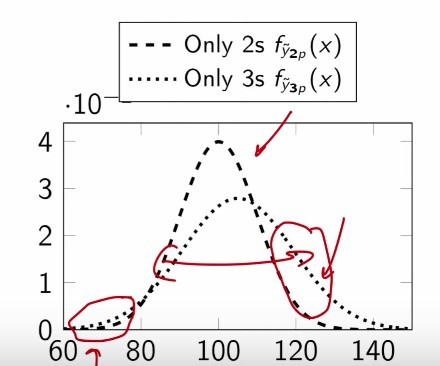
\includegraphics[widht=10cm]{notes/week_4/Video 2: THE CENTRAL LIMIT THEOREM/immages/v_2_2.jpg}
\item so the score difference looks like this \\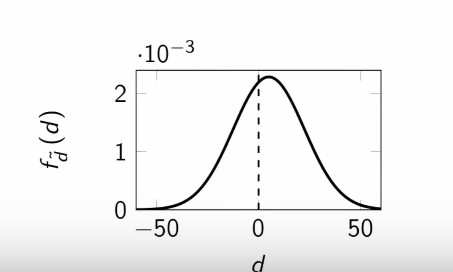
\includegraphics[widht=10cm]{notes/week_4/Video 2: THE CENTRAL LIMIT THEOREM/immages/v_2_3.jpg} 
\item then if we integrate the probability $d\geq 0$ then we can see that  the Gaussian animation of strategy 3 winning is .61
\item if we compare this to what we get with monte carlo simultaneous we get .6. so in other words the Gaussian approximation is really close and very easy to do 
\item naturally we also assumed Independence
\item so it more of a quick estimate
\section{implications of central limit theorem}
\subsection{distribution of the sample mean }
\item suppose we are us sing iid samples to calculate the sample mean as an estimator of of the sample mean 
\item the sample mean $\Tilde{m}_{n}=\frac{1}{n}\Sigma_{i=1}^{n}\Tilde{x}_i$
\item $E[\Tilde{m}_{n}]=\mu_{pop}$
\item and $var(\Tilde{m}_{n})=\frac{\sigma^2_{pop}}{n}$
\item and thus we have standard error $se(\Tilde{m}_{n})=\frac{\sigma_{pop}}{\sqrt{n}}$
\item further as $n\rightarrow \infty$ $\Tilde{m}_{n}$ converges in distribution to a Gaussian with mean $\mu_{pop}$ and standard deviation $se[\Tilde{m}_{n}]$

\end{itemize}
\end{document}
